\documentclass[border=10pt]{standalone}
\usepackage[svgnames]{xcolor}
\usepackage{amsmath}
\usepackage{pgfplots}
\pgfplotsset{compat=newest}
\usepackage[sfdefault]{FiraSans}
\usepackage{FiraMono}
\renewcommand*\familydefault{\sfdefault}
\begin{document}
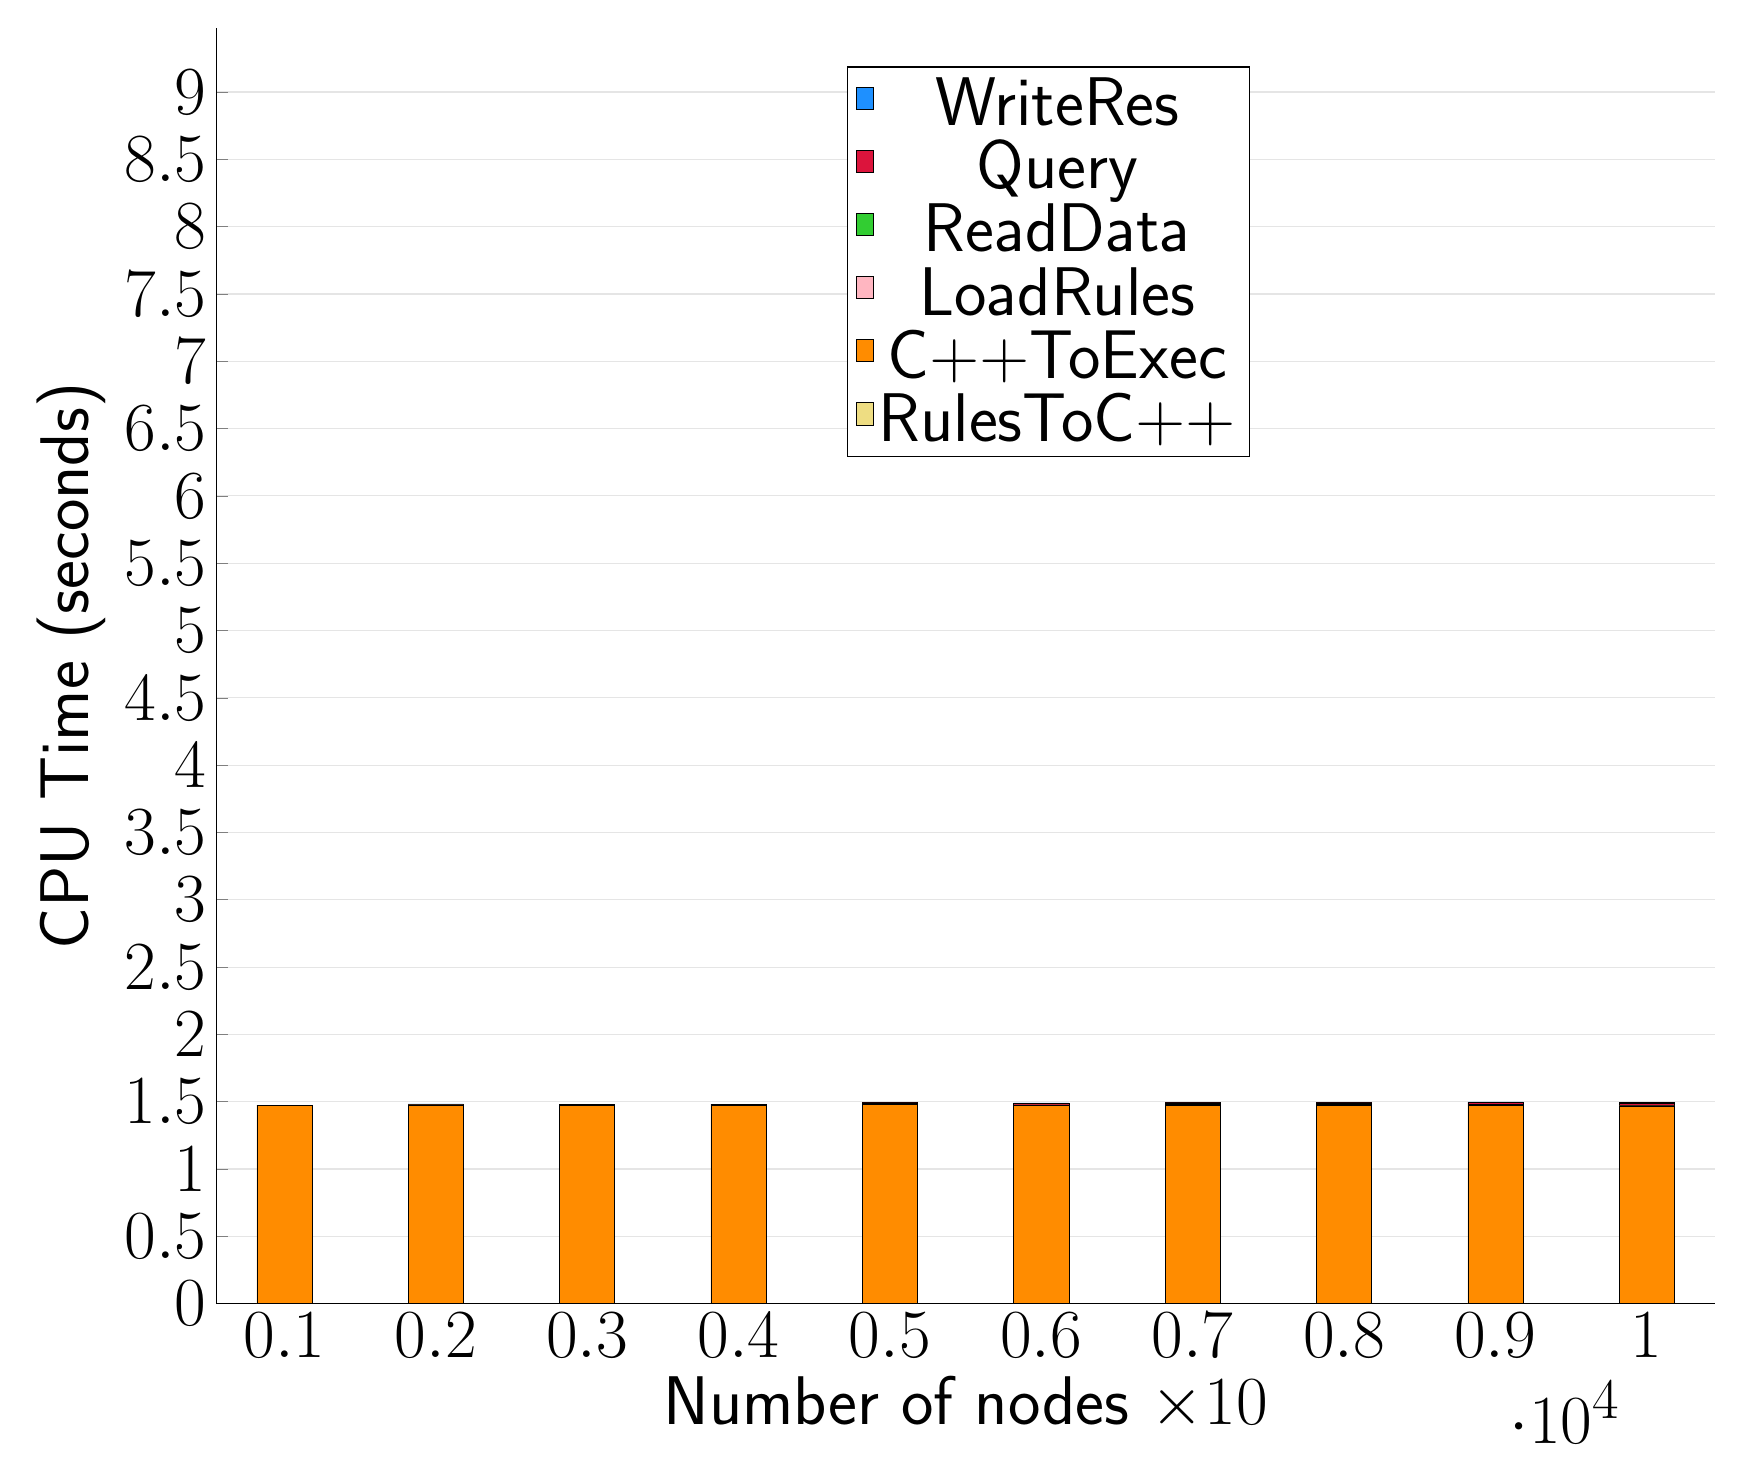
\begin{tikzpicture}
\begin{axis}[
   ybar stacked,
   width=1.7\textwidth,
   bar width=0.7cm,
   ymajorgrids, tick align=inside,
   major grid style={draw=gray!20},
   xtick=data,
   ymin=0, ymax=9.474,
   axis x line*=bottom,
   axis y line*=left,
   enlarge x limits=0.05,
   legend style={
       at={(0.69, 0.97)},
       anchor=north east,
       legend columns=1,
       font=\Huge,
   },
   ylabel={CPU Time (seconds)},
   xlabel={Number of nodes $\times 10$},
   label style={font=\Huge},
   tick label style={font=\Huge},
]
\addlegendimage{fill=DodgerBlue, draw=black, line width=0.2pt}
\addlegendentry{WriteRes}
\addlegendimage{fill=Crimson, draw=black, line width=0.2pt}
\addlegendentry{Query}
\addlegendimage{fill=LimeGreen, draw=black, line width=0.2pt}
\addlegendentry{ReadData}
\addlegendimage{fill=LightPink, draw=black, line width=0.2pt}
\addlegendentry{LoadRules}
\addlegendimage{fill=DarkOrange, draw=black, line width=0.2pt}
\addlegendentry{C++ToExec}
\addlegendimage{fill=LightGoldenrod, draw=black, line width=0.2pt}
\addlegendentry{RulesToC++}
\addplot +[fill=LightGoldenrod, draw=black, line width=0.2pt] coordinates {
(1000, 0.0)
(2000, 0.0)
(3000, 0.0)
(4000, 0.0)
(5000, 0.0)
(6000, 0.0020000000000000005)
(7000, 0.0)
(8000, 0.0020000000000000005)
(9000, 0.0020000000000000005)
(10000, 0.0)
};
\addplot +[fill=DarkOrange, draw=black, line width=0.2pt] coordinates {
(1000, 1.47)
(2000, 1.476)
(3000, 1.47)
(4000, 1.47)
(5000, 1.48)
(6000, 1.472)
(7000, 1.4739999999999998)
(8000, 1.472)
(9000, 1.472)
(10000, 1.4679999999999997)
};
\addplot +[fill=LightPink, draw=black, line width=0.2pt] coordinates {
(1000, 0.000165)
(2000, 0.0001642)
(3000, 0.0001712)
(4000, 0.0001698)
(5000, 0.0001744)
(6000, 0.0001586)
(7000, 0.0001716)
(8000, 0.00016779999999999999)
(9000, 0.00017039999999999997)
(10000, 0.00016219999999999999)
};
\addplot +[fill=LimeGreen, draw=black, line width=0.2pt] coordinates {
(1000, 0.0008768)
(2000, 0.0012958000000000002)
(3000, 0.0016435999999999998)
(4000, 0.0021039999999999995)
(5000, 0.0023736)
(6000, 0.0024898)
(7000, 0.0031219999999999998)
(8000, 0.0034785999999999997)
(9000, 0.0036101999999999996)
(10000, 0.0042524)
};
\addplot +[fill=Crimson, draw=black, line width=0.2pt] coordinates {
(1000, 0.002432)
(2000, 0.0044542)
(3000, 0.0063946)
(4000, 0.0076264)
(5000, 0.0092182)
(6000, 0.0106204)
(7000, 0.0135494)
(8000, 0.0138822)
(9000, 0.0158348)
(10000, 0.0176056)
};
\addplot +[fill=DodgerBlue, draw=black, line width=0.2pt] coordinates {
(1000, 0.0012824)
(2000, 0.0018894)
(3000, 0.0019129999999999998)
(4000, 0.0024427999999999997)
(5000, 0.0031726)
(6000, 0.0031392000000000004)
(7000, 0.0037242000000000004)
(8000, 0.0040414)
(9000, 0.0042452)
(10000, 0.004446199999999999)
};
\end{axis}
\end{tikzpicture}

\end{document}
